\documentclass[11pt,letterpaper]{article}
\usepackage[margin=2.5cm,top=3.5cm,bottom=3cm]{geometry}
\usepackage{booktabs}
\usepackage{graphicx}
\usepackage[hidelinks]{hyperref}
\usepackage{microtype}
\usepackage[table,dvipsnames]{xcolor}
\usepackage{longtable}
\usepackage{array}
\usepackage{caption}
\usepackage[T1]{fontenc}
\usepackage{lmodern}
\usepackage{fancyhdr}
\usepackage{amsmath}
\usepackage{titlesec}
\usepackage{enumitem}

\definecolor{wavblue}{RGB}{26,58,92}
\definecolor{wavgray}{RGB}{120,120,120}
\definecolor{wavlight}{RGB}{235,242,250}
\definecolor{wincolor}{RGB}{0,110,0}

\graphicspath{{/Users/egs/repos/waverider/benchmarks/canonical_tests/}}

\pagestyle{fancy}
\fancyhf{}
\fancyhead[L]{\small\color{wavgray}Manifold-Informed Architecture Benchmark \textemdash\ DERMATOLOGY}
\fancyhead[R]{\small\color{wavgray}\texttt{waverider @ 054030a}}
\fancyfoot[C]{\small\color{wavgray}\thepage}
\renewcommand{\headrulewidth}{0.4pt}

\titleformat{\section}{\large\bfseries\color{wavblue}}{}{0em}{}[\color{wavblue}\titlerule]
\titleformat{\subsection}{\normalsize\bfseries\color{wavblue}}{}{0em}{}
\setlength{\parindent}{0pt}
\setlength{\parskip}{4pt plus 1pt}

\begin{document}

\begin{center}
  {\LARGE\bfseries\color{wavblue} Manifold-Informed Architecture Benchmark}\\[6pt]
  {\large DERMATOLOGY: 6 classes, 34D input}\\[8pt]
  {\small Generated: 2026-04-15 09:41:13 \quad$|$\quad Apple M5 Max MacBook Pro, 64 GB RAM, 2TB SSD}\\[2pt]
  {\small\texttt{waverider @ 054030a} (--abbrev-re
054030a600978c0e9ffac58faf7157939927d009) \quad$|$\quad 2026-04-14 22:20:05 -0400}
\end{center}
{\color{wavblue}\noindent\rule{\linewidth}{1.5pt}}
\medskip

\noindent\colorbox{wavlight}{\parbox{\dimexpr\linewidth-2\fboxsep\relax}{
  \smallskip
  \textbf{Best:} Standard (256$\rightarrow$128)\quad test acc $= 0.9671 \pm 0.0205$\\[2pt]
  \textbf{Manifold:} 34D $\rightarrow$ 13D (61.8\%\ noise dimensions)\\[2pt]
  \smallskip
}}
\bigskip

\section{Experimental Setup}

\begin{tabular}{@{}ll@{}}
\toprule
\textbf{Parameter} & \textbf{Value} \\
\midrule
  Dataset & DERMATOLOGY \\
  Input dimensionality & 34D \\
  Classes & 6 \\
  Intrinsic dim ($d$) & 13 \\
  Variance threshold ($\tau$) & 0.9 \\
  Epochs & 50 \\
  Trials & 3 \\
  Batch size & 32 \\
  Learning rate & 0.001 \\
  $k$ neighbors (local PCA) & 40 \\
\bottomrule
\end{tabular}

\section{Manifold Discovery}

Local PCA over the training set, $k = 40$ neighbors. Intrinsic dimensionality $d$ is taken as the maximum per-class maximum at $\tau = 0.9$, clamped to $n_{\mathrm{classes}} = 6$.

\begin{tabular}{@{}rrrrrr@{}}
\toprule
$\tau$ & Mean $d$ & Std & Min & Max & Noise (\%) \\
\midrule
  0.95 & 13.9 & 1.4 & 11 & 17 & 59.2 \\
  0.90 & 11.4 & 1.2 & 8 & 13 & 66.6 \\
  0.85 & 9.7 & 1.2 & 6 & 12 & 71.6 \\
  0.80 & 8.4 & 1.1 & 4 & 10 & 75.2 \\
\bottomrule
\end{tabular}

\subsection{Per-Class Intrinsic Dimensionality}

\begin{tabular}{@{}lrrrr@{}}
\toprule
Class & Mean $d$ & Std & Min & Max \\
\midrule
  2 & 12.6 & 0.5 & 12 & 13 \\
  0 & 12.2 & 0.5 & 11 & 13 \\
  4 & 10.5 & 0.5 & 10 & 11 \\
  1 & 10.2 & 0.4 & 10 & 11 \\
  3 & 10.1 & 0.5 & 9 & 11 \\
  5 & 8.0 & 0.0 & 8 & 8 \\
\bottomrule
\end{tabular}

\section{Architecture Comparison}

{\small
\begin{tabular}{@{}p{7cm}rccr@{}}
\toprule
\textbf{Architecture} & \textbf{Params} & \textbf{Test Acc ($\mu \pm \sigma$)} & \textbf{Loss} & \textbf{Acc/Kparam} \\
\midrule
  {Euclidean KNN (k=7)} & 0 & $0.9590 \pm 0.0213$ & --- & --- \\
  {ManifoldModel ($\tau$=0.9)} & 0 & $0.9590 \pm 0.0151$ & --- & --- \\
  {\color{wincolor}Standard (256$\rightarrow$128)\,$\star$} & 42,630 & $0.9671 \pm 0.0205$ & 0.0918 & 0.0227 \\
  {Manifold (2d$\rightarrow$d, d=13)} & 539 & $0.9635 \pm 0.0198$ & 0.1380 & 1.7876 \\
  {Wide Manifold (d+1=14)} & 580 & $0.9654 \pm 0.0186$ & 0.1303 & 1.6644 \\
  {Manifold+ManifoldAdam (d=13)} & 539 & $0.9554 \pm 0.0202$ & 0.1547 & 1.7725 \\
  {PCA$\rightarrow$13D + MLP (2d$\rightarrow$d)} & 799 & $0.9580 \pm 0.0237$ & 0.1072 & 1.1990 \\
  {Intrinsic Dim (PCA$\rightarrow$13D$\rightarrow$C)} & 266 & $0.9444 \pm 0.0322$ & 0.2374 & 3.5504 \\
\bottomrule
\end{tabular}
}

\smallskip
{\small $\star$ = best performing architecture}

\section{Key Findings}

\begin{itemize}[leftmargin=*,itemsep=3pt]
  \item \textbf{Best architecture:} Standard (256$\rightarrow$128) \textemdash\ test accuracy $0.9671 \pm 0.0205$
  \item \textbf{Manifold compression:} 34D $\rightarrow$ 13D (61.8\%\ of ambient dimensions carry no structure)
\end{itemize}

\clearpage
\section{Result Figure}

\begin{figure}[htbp]
\centering
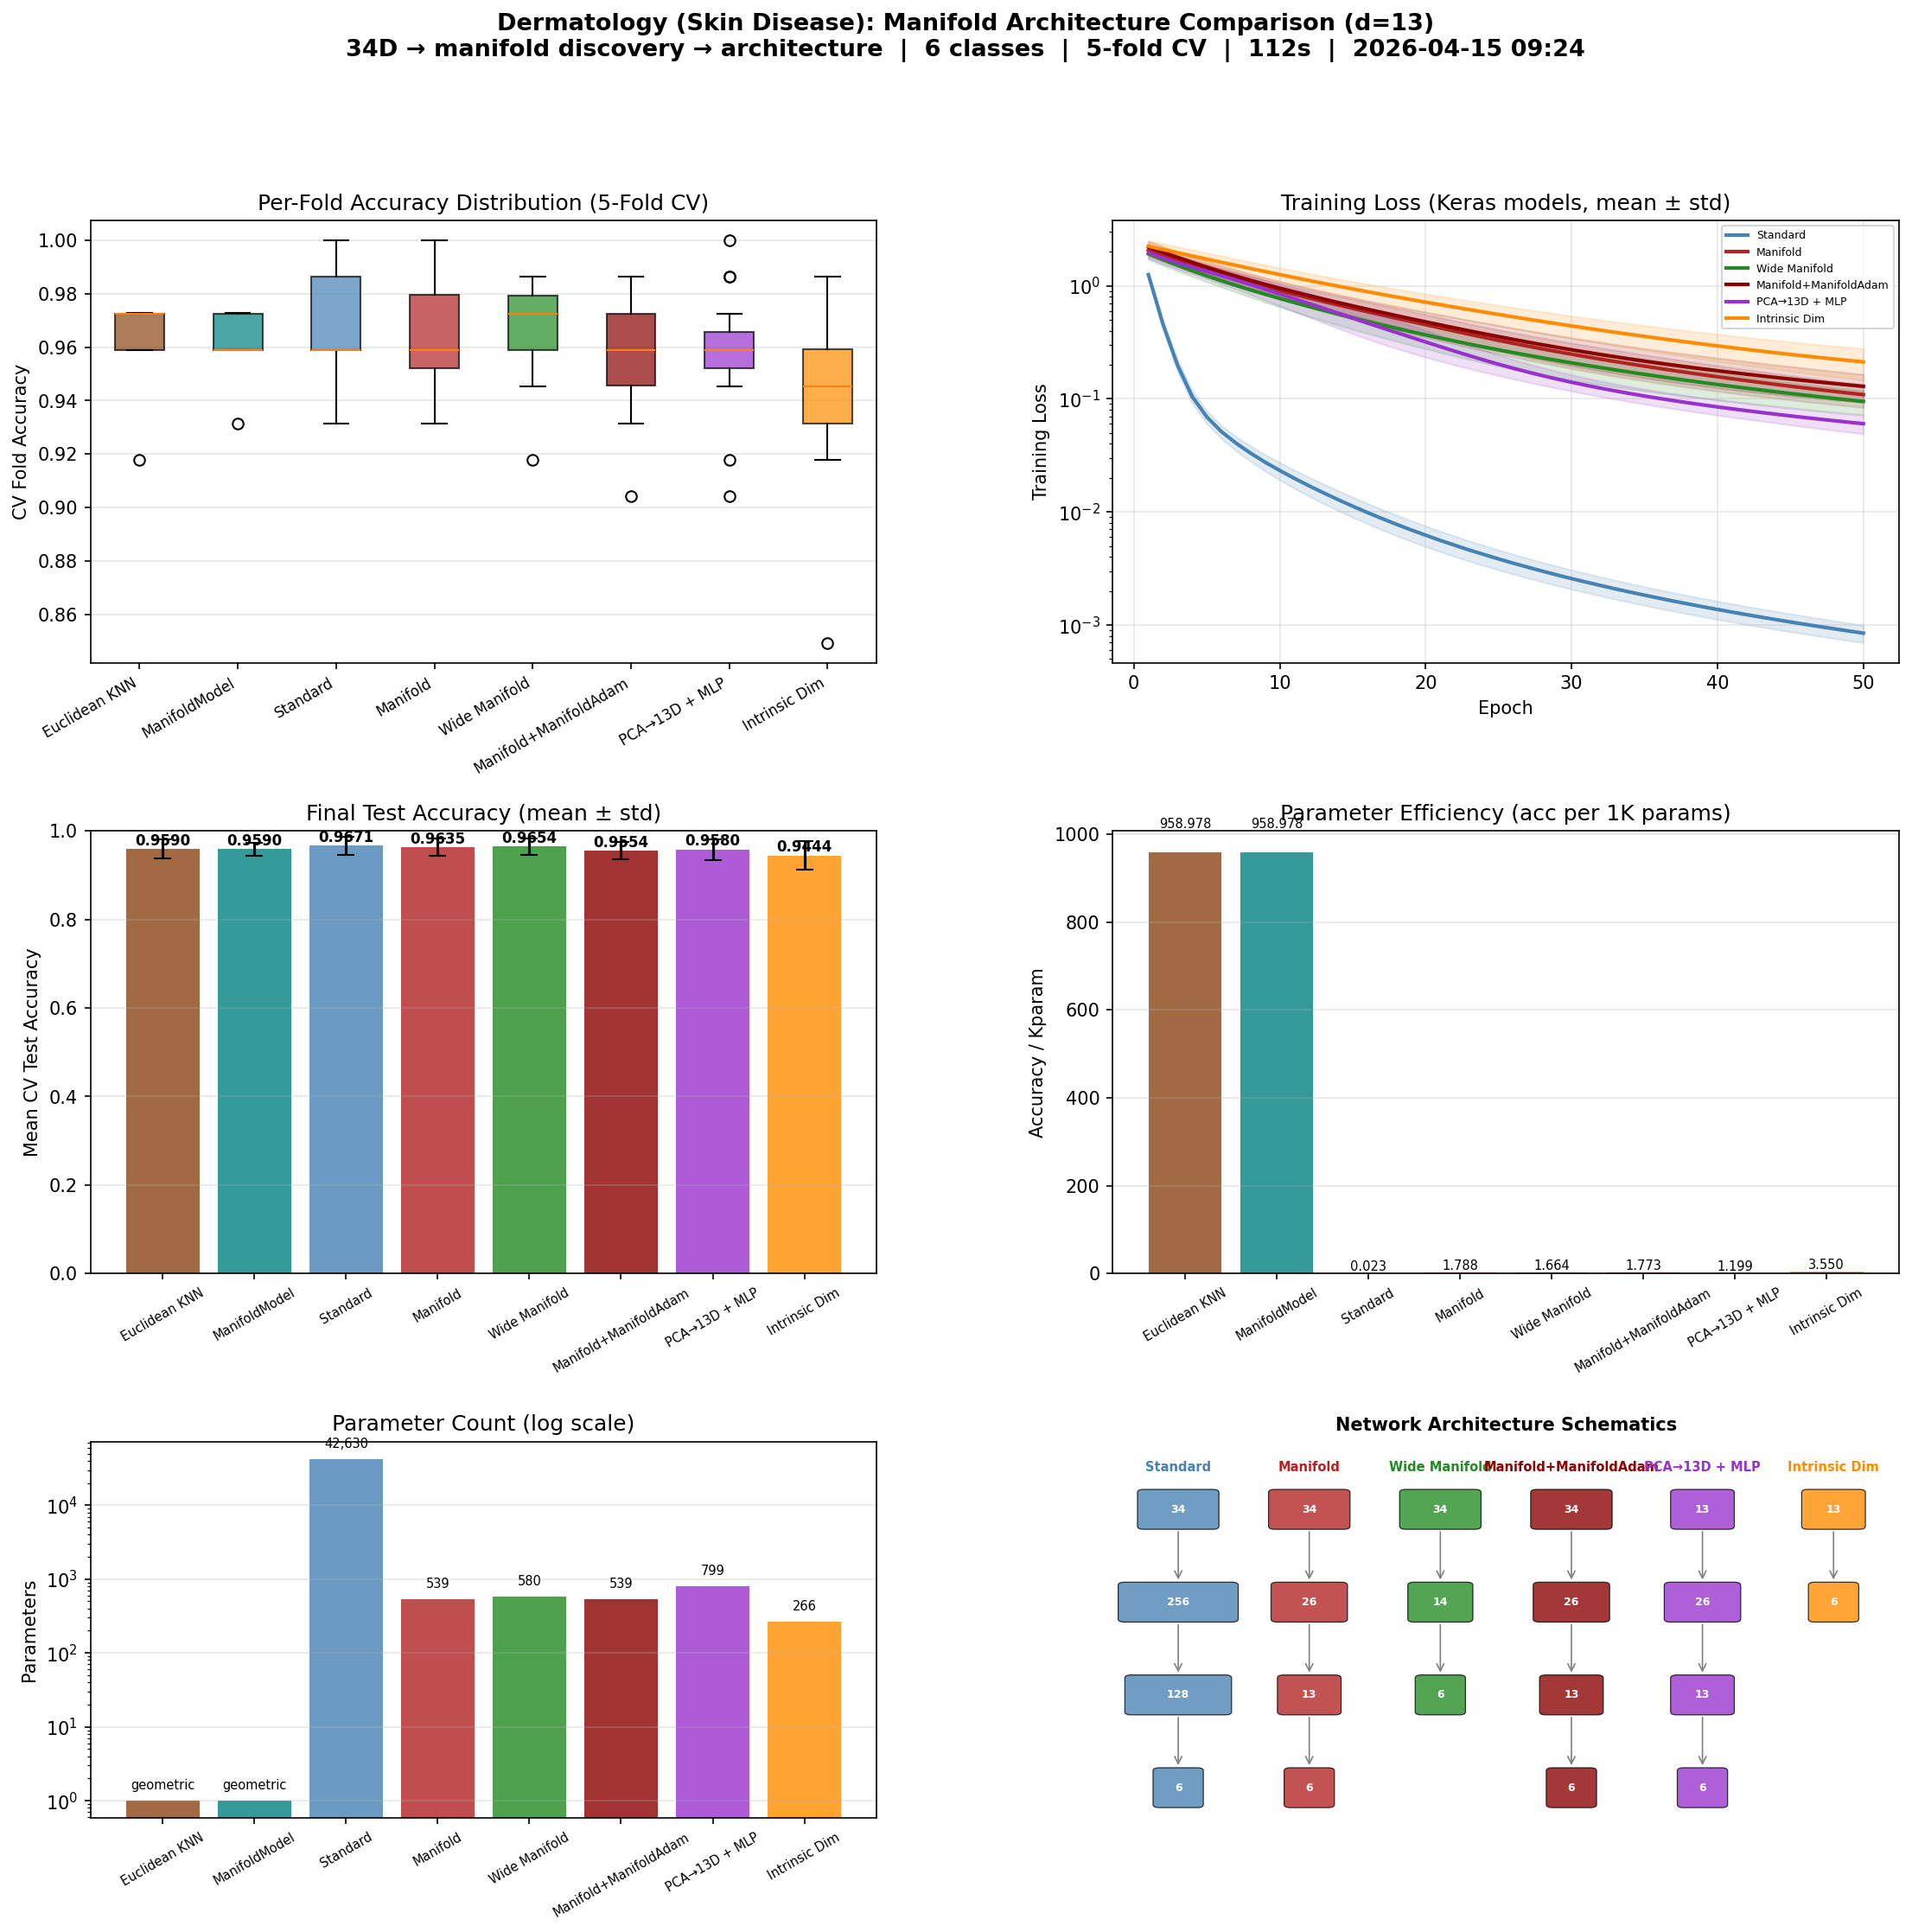
\includegraphics[width=\textwidth]{dermatology_disease_architecture_results}
\caption{DERMATOLOGY manifold-informed vs.\ standard architecture comparison. $d = 13$, 50 epochs, 3 trials.}
\end{figure}

\section{Provenance}

\begin{tabular}{@{}ll@{}}
\toprule
\textbf{Item} & \textbf{Value} \\
\midrule
  Repository & \href{https://github.com/Flux-Frontiers/waverider}{Flux-Frontiers/waverider} \\
  Commit & \texttt{054030a} (--abbrev-re
054030a600978c0e9ffac58faf7157939927d009) \\
  Commit date & 2026-04-14 22:20:05 -0400 \\
  Commit message & chore(release): bump version to 0.6.0 \\
  Python & 3.12.13 \\
  TensorFlow & 2.21.0 \\
  Device & CPU (forced) \\
  Host & Turing \\
  OS & macOS-26.4-arm64-arm-64bit \\
  Machine & Apple M5 Max MacBook Pro, 64 GB RAM, 2TB SSD \\
  Generated & 2026-04-15 09:41:13 \\
\bottomrule
\end{tabular}

\end{document}
